\section{Zustandsüberwachung}

Neben dem Anwendungsbereich der Regelungstechnik ist der Einsatz von Black-Box-Modellen ebenfalls im Bereich der Zustandsüberwachung denkbar. \\
Nach \cite{Isermann.2010} ergeben sich für die Zustandsüberwachung neben der Anzeige des gegenwärtigen Prozesszustandes ebenfalls die Meldung unerlaubter Betriebszustände und die Einleitung notwendiger Maßnahmen zur Einhaltung des Betriebs und zur Unfallvermeidung als Aufgabengebiete. \cite{Isermann.2010} unterscheidet dabei drei Arten der Überwachung:


\begin{itemize}
	\item \textit{Grenzwertüberwachung}: Nach Überschreiten von festgelegten Toleranzen durch gemessene Größen erzeugt das System Alarmmeldungen.
	\item \textit{Automatischer Schutz}: Bei der Entstehung von gefährlichen Prozesszuständen leitet die Grenzwertüberwachung Gegenmaßnahmen zur Überführung in einen sicheren Zustand ein. 
	\item \textit{Überwachung mit Fehlerdiagnose:} Merkmale werden aus messbaren Größen abgeleitet, daraus Symptome erzeugt, Fehlerdiagnosen durchgeführt und Gegenmaßnahmen eingeleitet. \cite{Isermann.2010}
\end{itemize} 
  
Nach \cite{Isermann.2010} eignen sich die ersten beiden Methoden vor allem für stationäre Prozesse, da bei diesen die Definition eines eng anliegenden Toleranzbandes um die Prozessgröße herum möglich ist. Diese zeichnen sich durch eine hohe Zuverlässigkeit und Einfachheit aus. \cite{Isermann.2010} \\
Mit den ersten beiden Methoden ist es jedoch kaum möglich, Prozesse in dynamischen Betriebszuständen zu überwachen, da dabei große Veränderungen der Prozessgrößen entstehen. Beispielsweise würde dabei ein für einen stationären Prozess ausgelegtes Toleranzband überschritten werden, was zu einem Fehlalarm führen könnte. Zudem eignen sich die ersten beiden Methoden nicht zum frühzeitigen Erkennen kleiner Fehler, da dabei das Toleranzband nicht überschritten würde. Auch bleiben der Fehlerort, die Fehlergröße und die Fehlerursache unberücksichtigt. Aus diesen Gründen ist die Weiterentwicklung der dritten Methode, die Überwachung mit integrierter Fehlerdiagnose, notwendig \cite{Isermann.2010}. \\

Nach \cite{Isermann.2010} ist für die Fehlerdiagnose das Erkennen von sogenannten Symptomen entscheidend. Ein Symptom entspricht der Differenz zwischen dem beobachteten und dem normalen Merkmal. Je nachdem, ob es sich um ein Signal- oder um ein Prozessmodell handelt, können Merkmale entweder Schwellenwertüberschreitungen, Amplituden und Frequenzen (bei Signalmodellen) oder Parameter, Zustandsvariablen und Residuen (bei Prozessmodellen) sein, siehe Abbildung \ref{fig:symptome}. \cite{Isermann.2010}

\begin{figure} 
	\centering
	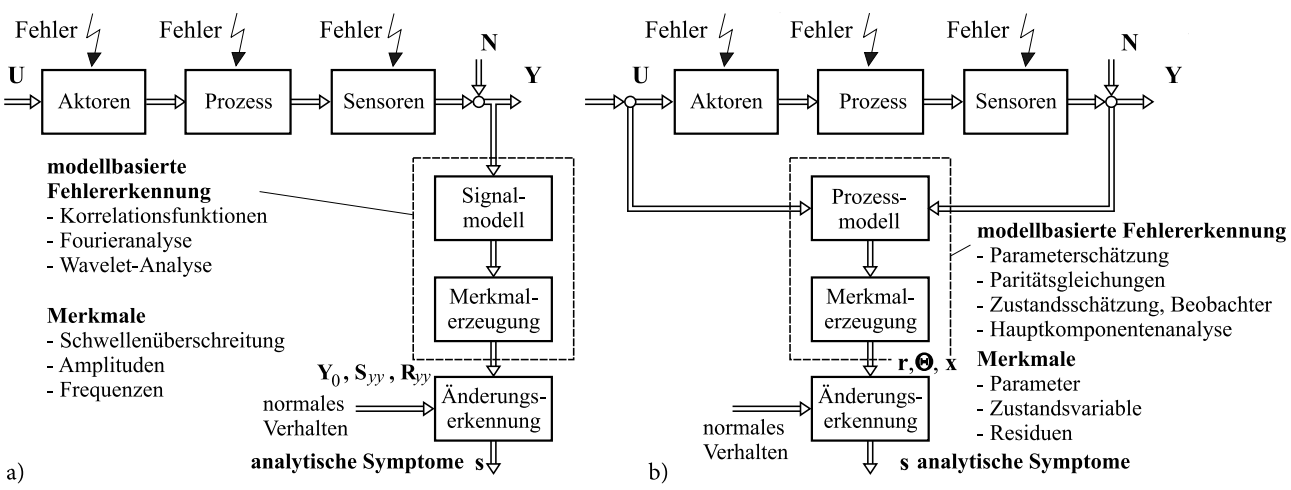
\includegraphics[width=1.0\textwidth]{images/symptome}
	\caption{Fehlererkennung mit Signal- und Prozessmodellen (a) signalmodellbasiert, (b) prozessmodellbasiert. \cite{Isermann.2010}}
	\label{fig:symptome}
\end{figure}



In beiden Fällen findet ein Vergleich der Merkmale mit den normalen Merkmalen des fehlerlosen Prozesses statt. Mit Hilfe von Methoden zur Erkennung signifikanter Änderungen (z.B. Parameterabschätzung, Paritätsgleichungen, Zustandsgrößenbeobachter, neuronale Netzwerke, etc.) können so die \textit{analytischen Symptome} ermittelt werden, siehe Abbildung \ref{fig:fehlererkennungsmethoden}. \cite{Isermann.2010}

\begin{figure} 
	\centering
	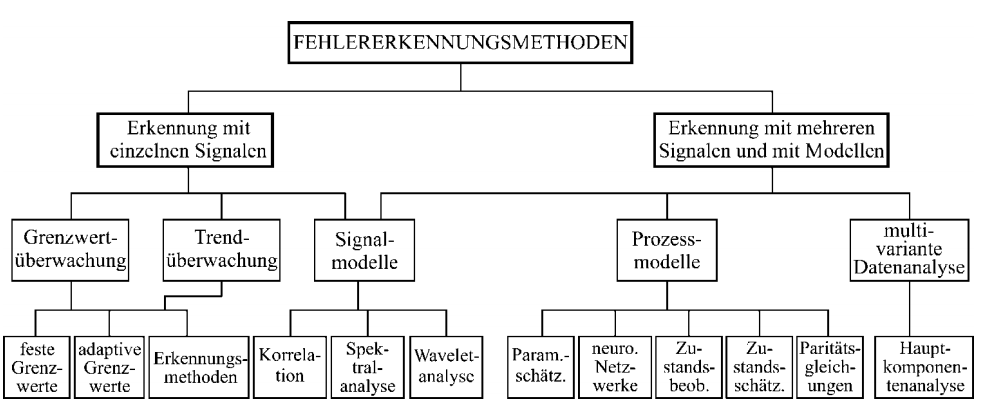
\includegraphics[width=0.85\textwidth]{images/fehlererkennungsmethoden}
	\caption{Übersicht der Fehlererkennungsmethoden \cite{Isermann.2010}}
	\label{fig:fehlererkennungsmethoden}
\end{figure}



Im weiteren Verlauf findet die Ermittlung des Zusammenhangs zwischen den analytischen Symptomen und den Fehlern entweder durch Klassifikationsmethoden (statistisch, geometrisch, Neuronale Netze, Fuzzy Cluster) oder durch Interferenzmethoden (Kausales Netz, Fehler-Symptom-Baum) statt. \cite{Isermann.2010}
 
Damit lässt sich sagen, dass Neuronale Netze im Bereich der Zustandsüberwachung zwei Anwendungsgebiete einnehmen. Zum einen können neuronale Netze als Prozessmodell zwecks Fehlererkennung fungieren. Zum Beispiel kann das neuronale Netz mit einem realen Prozesseingangssignal beaufschlagt werden. Bei einem fehlerhaften Prozess würde das vom neuronalen Netz herausgegebene Ausgangssignal sich vom  Ausgangssignal eines normalen Prozesses unterscheiden. Weiterhin kann das neuronale Netz als Klassifikationsmethode genutzt werden, um bereits ermittelte \textit{analytische Symptome} mit Fehlern in einen Zusammenhang zu bringen.  




 